\documentclass[aspectratio=169]{beamer}

% UGM Presentation Theme-like setup
\usetheme{Madrid}
\usecolortheme{dolphin}
\usefonttheme{professionalfonts}

% Custom Colors (UGM Gold/Blue inspiration)
\definecolor{ugmblue}{RGB}{0, 50, 100}
\setbeamercolor{structure}{fg=ugmblue}

\usepackage[utf8]{inputenc}
\usepackage[T1]{fontenc}
\usepackage[indonesian]{babel}
\usepackage{amsmath}
\usepackage{booktabs}
\usepackage{graphicx}
\usepackage{listings}
\usepackage{xcolor}
\usepackage{bytefield}

% Style for code blocks
\lstset{
  basicstyle=\ttfamily\scriptsize,
  breaklines=true,
  frame=single,
  backgroundcolor=\color{gray!10},
  keywordstyle=\color{ugmblue},
  commentstyle=\color{green!50!black},
  stringstyle=\color{red!70!black},
}

% ── colour shortcuts ──────────────────────────────────────────
\newcommand{\good}[1]{\textcolor{green!60!black}{\textbf{#1}}}
\newcommand{\bad}[1]{\textcolor{red!70!black}{\textbf{#1}}}
\newcommand{\reg}[1]{\texttt{\small #1}}

\title{Perancangan IP I2S TX AXI4-Lite\\pada SoC MicroBlaze V}
\subtitle{Implementasi pada FPGA Basys3 dengan DAC PCM5102A\\
          \small Termasuk Identifikasi dan Perbaikan Bug Firmware}
\author{Nama Mahasiswa \\ NIM}
\institute{Departemen Teknik Elektro dan Teknologi Informasi\\Universitas Gadjah Mada}
\date{Mei 2026}

\begin{document}

% ── TITLE ─────────────────────────────────────────────────────
\begin{frame}
  \titlepage
\end{frame}

% ── OUTLINE ───────────────────────────────────────────────────
\begin{frame}{Outline}
  \tableofcontents
\end{frame}

%==============================================================
\section{Pendahuluan}
%==============================================================

\begin{frame}{Latar Belakang}
  \begin{itemize}
    \item Sistem embedded audio membutuhkan antarmuka serial yang \textbf{stabil, presisi,
          dan dapat dikonfigurasi dari perangkat lunak}.
    \item \textbf{I2S} (Philips, 1986) adalah standar de-facto untuk transmisi audio
          digital antarchip: BCLK, WS/LRCK, DATA.
    \item \textbf{AXI4-Lite} memungkinkan prosesor mengakses register peripheral
          melalui model \textit{memory-mapped I/O} yang sederhana.
    \item \textbf{MicroBlaze V} (RISC-V soft-core) pada ekosistem AMD/Xilinx
          menyediakan fondasi SoC yang terintegrasi dengan Vivado dan Vitis.
    \item Penelitian ini merancang IP I2S TX kustom, mengintegrasikannya ke SoC,
          \textbf{dan mendokumentasikan bug firmware} yang ditemukan selama validasi.
  \end{itemize}
\end{frame}

\begin{frame}{Rumusan Masalah dan Tujuan}
  \begin{columns}[T]
    \column{0.5\textwidth}
      \textbf{Rumusan Masalah}
      \begin{enumerate}\small
        \item Bagaimana merancang IP I2S TX dengan AXI4-Lite yang
              dapat diakses melalui register \textit{memory-mapped}?
        \item Bagaimana mendukung dua mode $F_s$ (48/96 kHz) dari
              satu sumber \texttt{audio\_clk}?
        \item Bagaimana memverifikasi fungsionalitas dan timing
              melalui ILA dan uji audio PCM5102A?
      \end{enumerate}
    \column{0.5\textwidth}
      \textbf{Batasan Penelitian}
      \begin{itemize}\small
        \item TX-only, format Philips I2S, stereo.
        \item Bare-metal (tanpa RTOS/Linux).
        \item Tanpa DMA dan tanpa FIFO internal.
        \item Platform: Basys3 (Artix-7) + PCM5102A.
        \item \textit{Programmed I/O} berbasis register murni.
      \end{itemize}
  \end{columns}
\end{frame}

%==============================================================
\section{Dasar Teori}
%==============================================================

\begin{frame}{Protokol I2S -- Philips Standard}
  \begin{columns}[T]
    \column{0.55\textwidth}
      \begin{itemize}
        \item \textbf{BCLK}: clock serial, \textit{sampling} data pada tepi naik.
        \item \textbf{WS}: LOW = kanal kiri; HIGH = kanal kanan.
        \item \textbf{DATA}: serial MSB-first; satu \textbf{delay bit} (selalu 0)
              setelah setiap peralihan WS.
        \item Satu frame stereo = \textbf{64 BCLK}
              (32 bit kiri + 32 bit kanan).
        \item DATA berubah pada tepi \textit{turun} BCLK; DAC membaca
              pada tepi \textit{naik}.
      \end{itemize}
    \column{0.45\textwidth}
      \IfFileExists{contents/figures/i2s-ip-block.png}{%
        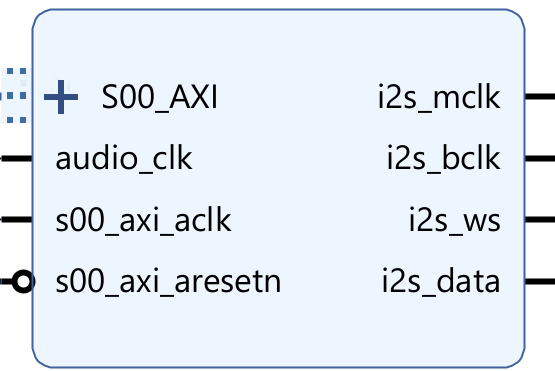
\includegraphics[width=\linewidth]{contents/figures/i2s-ip-block.png}%
      }{}
  \end{columns}
\end{frame}

%==============================================================
\section{Perancangan Sistem}
%==============================================================

\begin{frame}{Arsitektur Sistem -- Block Design}
  \begin{columns}[T]
    \column{0.50\textwidth}
      \begin{itemize}
        \item \textbf{MicroBlaze V} sebagai AXI master.
        \item \textbf{Clocking Wizard} menghasilkan 3 clock:\\
              100 MHz (AXI), 24,6 MHz (48k), 22,4 MHz (44,1k).
        \item \textbf{IP I2S} menerima data lewat register AXI4-Lite.
        \item Output PMOD JA → \textbf{PCM5102A}.
      \end{itemize}
    \column{0.50\textwidth}
      \IfFileExists{contents/figures/clocking-view-block-diagram.png}{%
        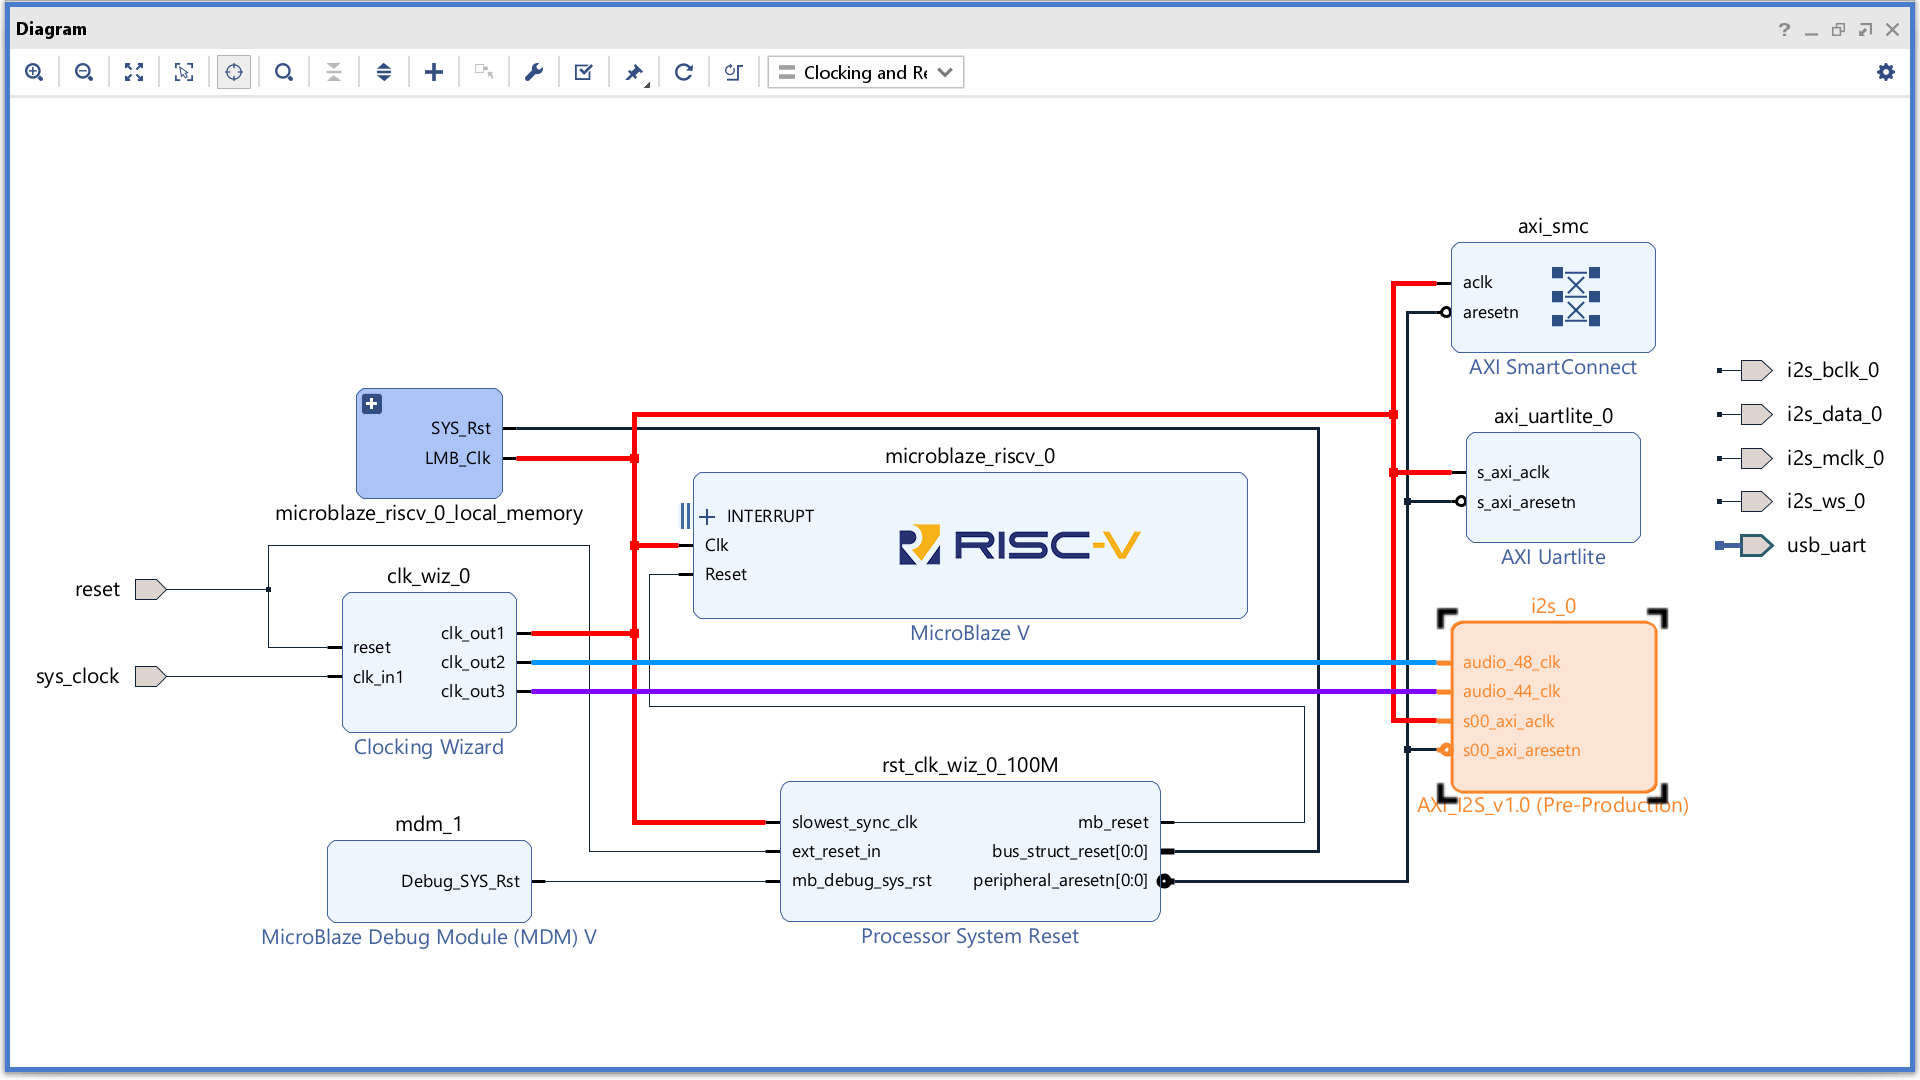
\includegraphics[width=\linewidth]{contents/figures/clocking-view-block-diagram.png}%
      }{}
  \end{columns}
\end{frame}

\begin{frame}{Resource Utilization \& Power Analysis}
  \begin{columns}[T]
    \column{0.50\textwidth}
      \textbf{Resource Utilization (Basys3):}
      \IfFileExists{contents/figures/utilization-summary.png}{%
        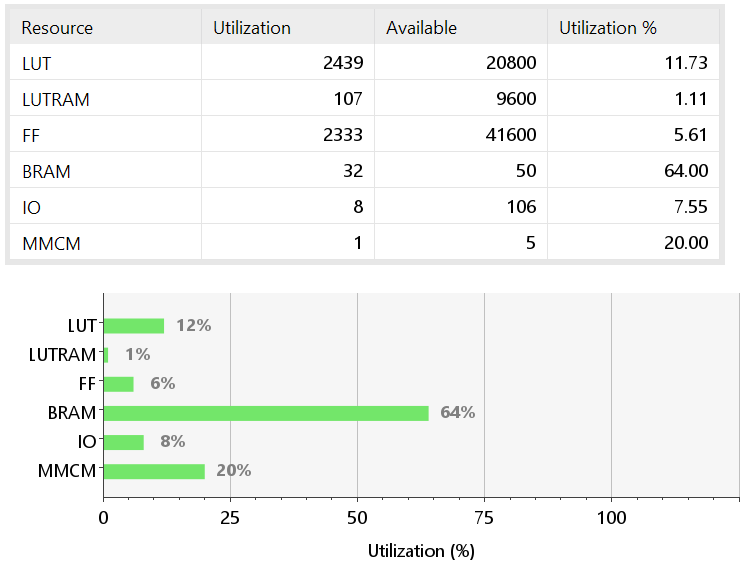
\includegraphics[width=\linewidth]{contents/figures/utilization-summary.png}%
      }{}
    \column{0.50\textwidth}
      \textbf{Power Analysis:}
      \IfFileExists{contents/figures/power-summary.png}{%
        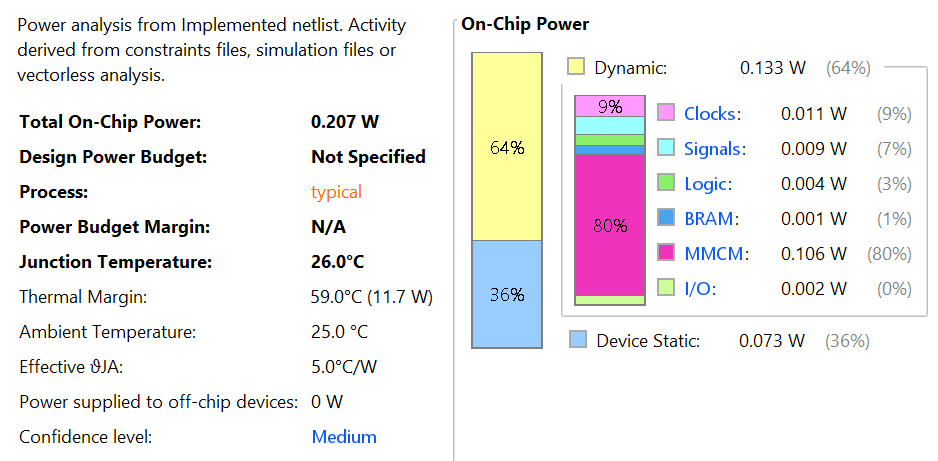
\includegraphics[width=\linewidth]{contents/figures/power-summary.png}%
      }{}
  \end{columns}
\end{frame}

%==============================================================
\section{Animasi Alur Logika I2S}
%==============================================================

\begin{frame}{Animasi: Serialisasi Philips I2S}
  \begin{center}
    \fbox{
      \begin{minipage}{0.8\textwidth}
        \centering
        \vspace{2em}
        [Animasi Manim: SerializationScene]\\
        Menunjukkan MSB-first dan One-bit delay\\
        \vspace{2em}
      \end{minipage}
    }
  \end{center}
  \begin{itemize}
    \item \textbf{WS Transition:} Penanda kanal kiri (LOW) ke kanan (HIGH).
    \item \textbf{One-bit Delay:} Bit pertama setelah transisi WS selalu 0.
    \item \textbf{Data Shift:} Mengirim 32 bit per slot per kanal.
  \end{itemize}
\end{frame}

%==============================================================
\section{Identifikasi dan Perbaikan Bug}
%==============================================================

\begin{frame}[fragile]{Bug 3: Presisi Timing Loop}
  \textbf{Penyebab:} \texttt{usleep()} tidak akumulatif dan memiliki granularitas rendah (~1 $\mu$s).
  
  \begin{columns}[T]
    \column{0.5\textwidth}
      \textbf{\bad{Metode Lama (Sleep):}}
\begin{lstlisting}[language=C]
uint32_t period_us = 1000000/Fs;
usleep(period_us - 2);
// Error terakumulasi tiap iterasi
\end{lstlisting}
    \column{0.5\textwidth}
      \textbf{\good{Metode Baru (Deadline):}}
\begin{lstlisting}[language=C]
uint64_t deadline = rdcycle64();
while(1) {
  stream_sample();
  deadline += period_cycles;
  while(rdcycle64() < deadline);
}
\end{lstlisting}
  \end{columns}
  \vspace{0.5em}
  \textit{Hasil: Frekuensi 1k/2k/5kHz tepat sasaran dengan presisi 10 ns (100 MHz clock).}
\end{frame}

%==============================================================
\section{Hasil Pengujian}
%==============================================================

\begin{frame}{Hasil Verifikasi Audio PCM5102A}
  \begin{columns}[T]
    \column{0.33\textwidth}
      \centering \textbf{Left Only}
      \IfFileExists{contents/figures/left-channel-only.jpeg}{%
        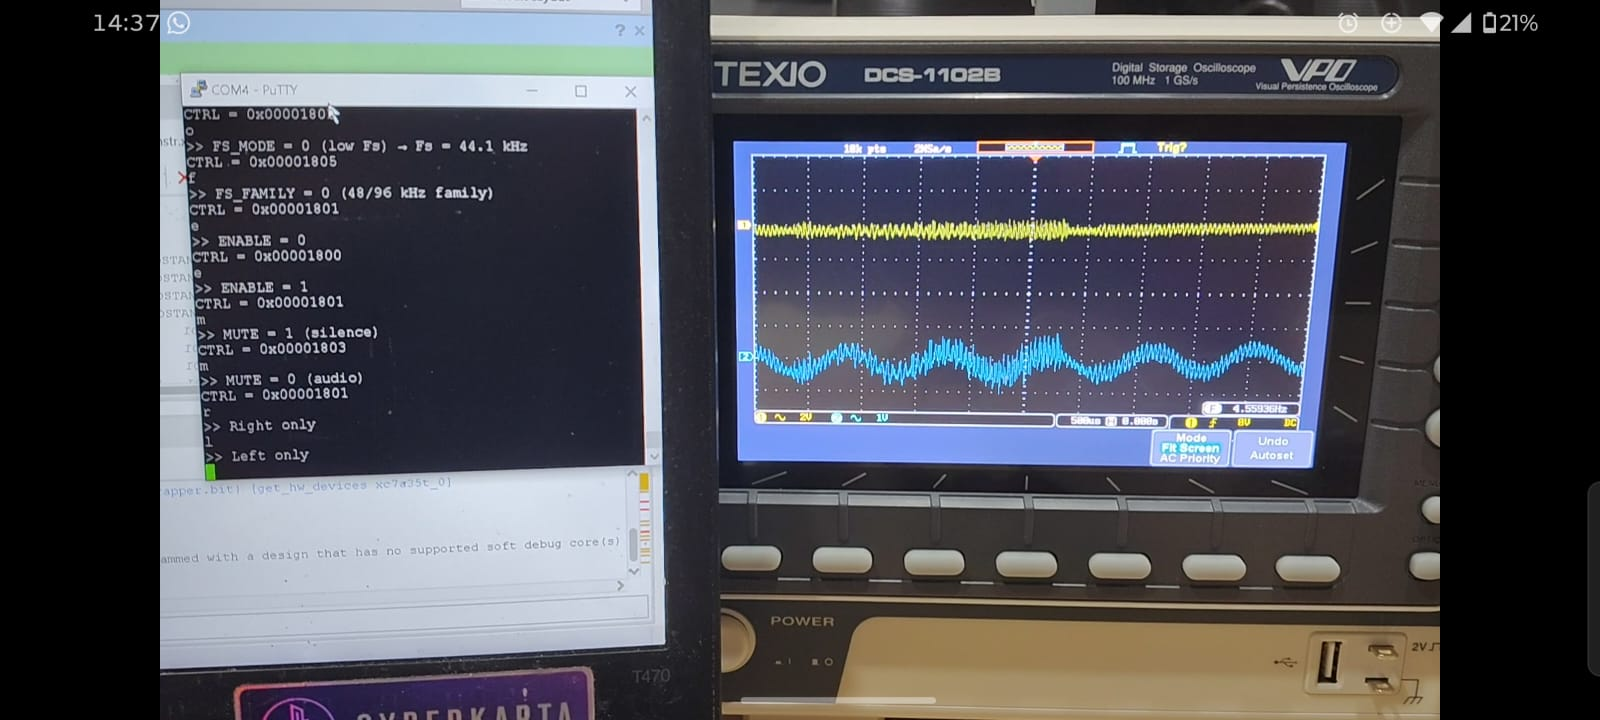
\includegraphics[width=\linewidth]{contents/figures/left-channel-only.jpeg}%
      }{}
    \column{0.33\textwidth}
      \centering \textbf{Right Only}
      \IfFileExists{contents/figures/right-channel-only.jpeg}{%
        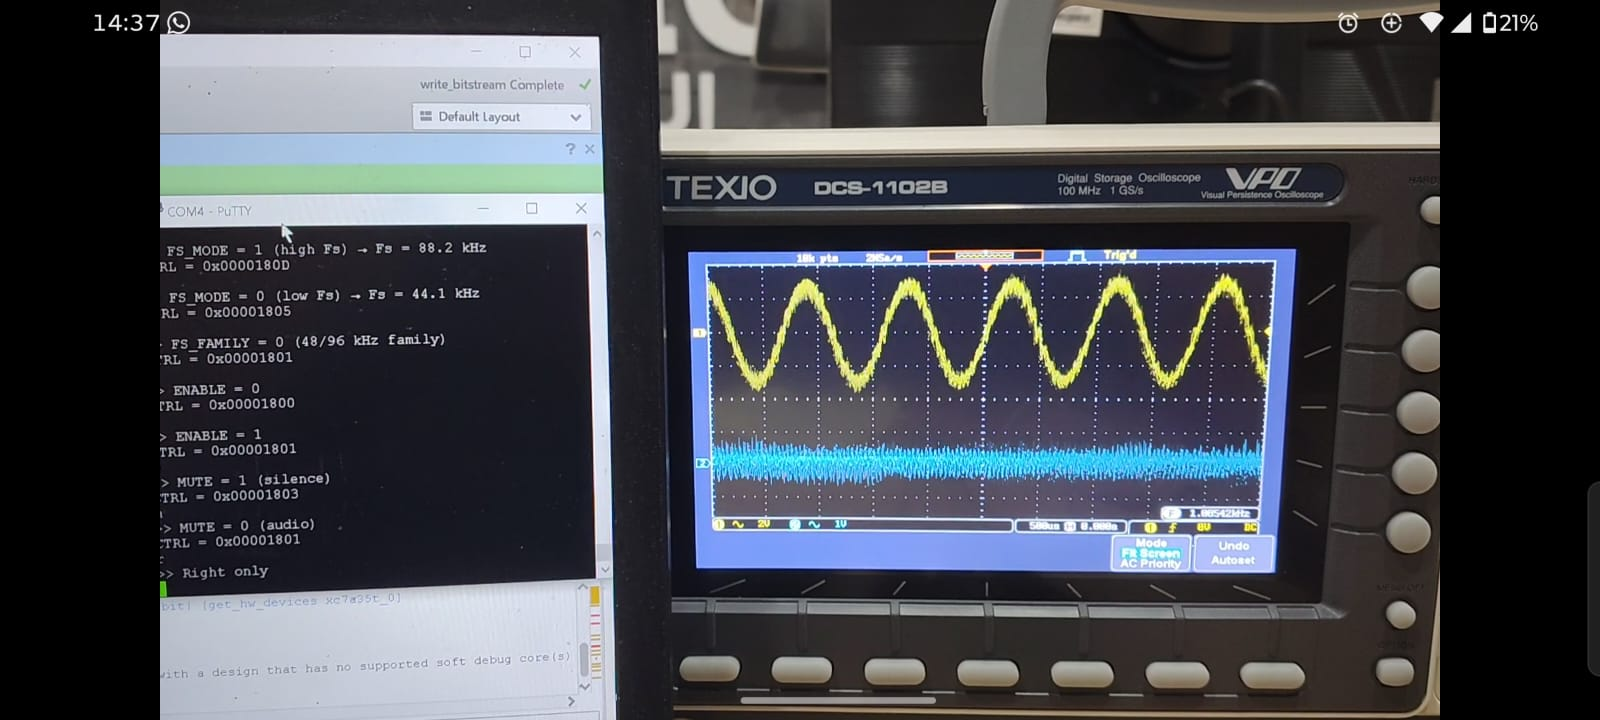
\includegraphics[width=\linewidth]{contents/figures/right-channel-only.jpeg}%
      }{}
    \column{0.33\textwidth}
      \centering \textbf{Both Channels}
      \IfFileExists{contents/figures/both-channel.jpeg}{%
        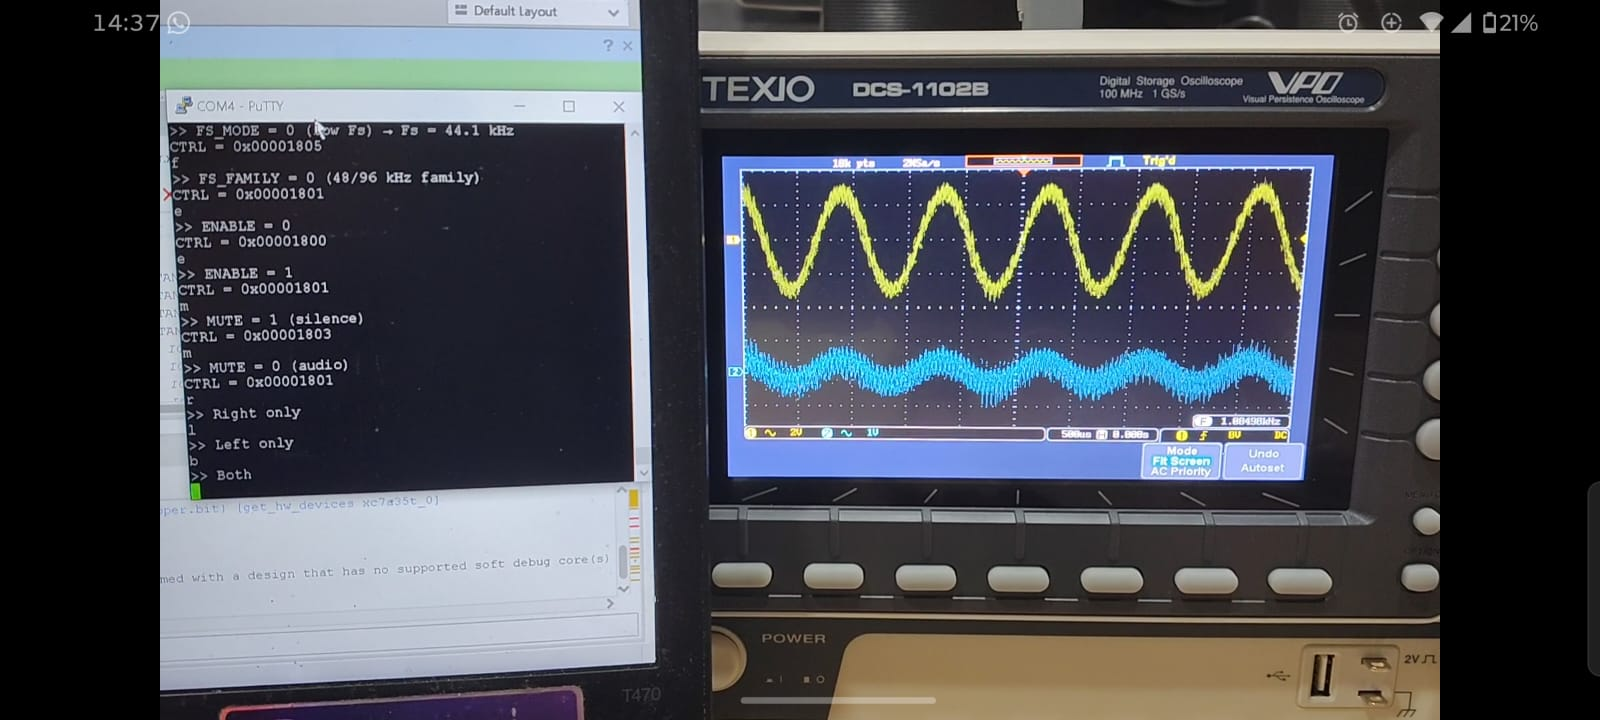
\includegraphics[width=\linewidth]{contents/figures/both-channel.jpeg}%
      }{}
  \end{columns}
\end{frame}

%==============================================================
\section{Penutup}
%==============================================================

\begin{frame}{Kesimpulan}
  \begin{enumerate}
    \item IP I2S TX AXI4-Lite berhasil diintegrasikan pada SoC MicroBlaze V.
    \item Dua mode $F_s$ (48/96 kHz) tervalidasi via hardware.
    \item Bug firmware (masking & timing) diperbaiki sepenuhnya di software.
    \item Validasi audio PCM5102A menunjukkan hasil yang presisi dan stabil.
  \end{enumerate}
\end{frame}

\begin{frame}{Terima Kasih}
  \centering
  \vspace{1em}
  {\Large \textbf{Terima Kasih}}
  \vspace{1.5em}
  \begin{block}{Kontribusi}
    \begin{itemize}
      \item IP core I2S TX AXI4-Lite (Verilog)
      \item Firmware optimasi timing RISC-V CSR
      \item Dokumentasi lengkap perbaikan bug
    \end{itemize}
  \end{block}
\end{frame}

\end{document}
